\chapter{Modelos Estudiados}
\label{chapter:modelos_estudiados}

Este capítulo presenta en detalle los dos modelos computacionales que constituyen los pilares conceptuales del presente trabajo. El modelo de \citeauthor{cuppini2017biologically} aborda la integración audiovisual y la inferencia causal mediante una arquitectura neuronal biológicamente inspirada, representando el objetivo a largo plazo hacia el cual apuntan las extensiones futuras de este trabajo. Y en la otra mano el modelo de \citeauthor{echeveste2020cortical} demuestra cómo circuitos corticales con restricciones biológicas pueden implementar inferencia probabilística mediante muestreo, exhibiendo dinámicas realistas como oscilaciones gamma y transitorios inhibitorios. Este segundo modelo constituye el objeto central de implementación del presente trabajo.

% =============================================================================
% SECCIÓN 1: EL MODELO DE CUPPINI
% =============================================================================

\section{El modelo de Cuppini para integración audiovisual e inferencia causal}
\label{sec:modelo_cuppini}

El problema de la inferencia causal multisensorial descripto en la Sección~\ref{subsec:inferencia_causal} ha motivado el desarrollo de diversos modelos computacionales. Entre ellos, el modelo desarrollado por \citet{cuppini2017biologically} representa un avance significativo al abordar específicamente la integración audiovisual y el efecto ventrílocuo mediante una arquitectura neuronal biológicamente inspirada.

\subsection{Arquitectura del modelo}
\label{subsec:cuppini_arquitectura}

El modelo se estructura en tres capas jerárquicas interconectadas, cada una compuesta por neuronas organizadas topográficamente según la posición espacial de su campo receptivo.

La \textbf{capa auditiva} procesa información sobre la localización espacial de estímulos sonoros. Cada unidad en esta capa responde preferentemente a sonidos provenientes de una posición específica del espacio, aunque con campos receptivos relativamente amplios que reflejan la menor precisión espacial de la audición comparada con la visión.

La \textbf{capa visual} procesa información sobre la localización de estímulos visuales. Las unidades en esta capa tienen campos receptivos más estrechos que sus contrapartes auditivas, capturando la mayor resolución espacial del sistema visual.

La \textbf{capa multisensorial} (o de inferencia causal) recibe proyecciones feedforward de ambas capas unisensoriales y computa la integración de señales y la decisión sobre la estructura causal subyacente.

Las capas se interconectan mediante tres tipos de sinapsis: conexiones \textit{laterales intra-área} organizadas en un perfil de ``sombrero mexicano'' que implementa competencia local, conexiones \textit{cross-modales} excitatorias recíprocas entre las capas auditiva y visual, y proyecciones \textit{feedforward} hacia la capa multisensorial.

\begin{figure}[!ht]
    \centering
    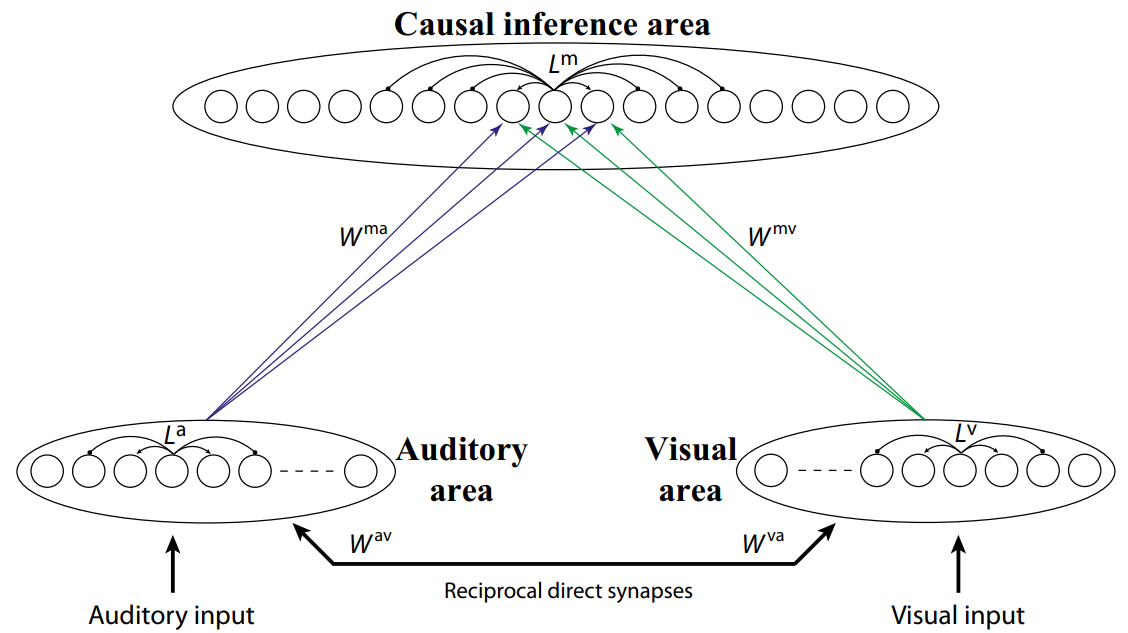
\includegraphics[width=0.95\textwidth]{04_antecedentes/figures/cuppini.png}
    \caption{
        Estructura de la red de \citeauthor{cuppini2017biologically}. Las regiones visual y auditiva procesan los estímulos sensoriales externos. Estas regiones están interconectadas mediante sinapsis excitatorias directas y envían proyecciones feedforward de largo alcance dirigidas al área de inferencia causal.
    }
    \label{fig:patterns/template_method}
\end{figure}

\subsection{Mecanismos de integración e inferencia}
\label{subsec:cuppini_mecanismos}

El modelo implementa dos mecanismos computacionales distintos pero interrelacionados:

El primer mecanismo, mediado por las \textbf{sinapsis cross-modales} entre las capas unisensoriales, produce la integración clásica multisensorial. Cuando estímulos visual y auditivo se presentan en posiciones espaciales cercanas, las conexiones cross-modales excitatorias refuerzan mutuamente las actividades en ambas regiones, atrayendo las representaciones espaciales hacia una posición común. Este mecanismo da lugar al efecto ventrílocuo: el sesgo de la localización auditiva percibida hacia la posición del estímulo visual.

El segundo mecanismo, mediado por la \textbf{capa multisensorial}, computa la inferencia causal propiamente dicha. La actividad en esta capa integra información de ambas modalidades y determina si los estímulos se perciben como provenientes de una causa común o de fuentes independientes. La presencia de uno o dos picos de actividad por encima de un umbral de detección indica, respectivamente, la inferencia de una causa única o de causas separadas.

\subsection{Capacidades y limitaciones}
\label{subsec:cuppini_limitaciones}

El modelo reproduce exitosamente varios fenómenos experimentales: \textbf{el efecto ventrílocuo} emerge naturalmente de la dinámica, con magnitud dependiente de la confiabilidad relativa de las señales; \textbf{el juicio de unidad} exhibe el patrón correcto donde la probabilidad de percibir una causa común disminuye con la disparidad espacial; y el \textbf{sesgo auditivo} es modulado por la decisión causal, siendo mayor cuando se infiere una causa común \citep{cuppini2017biologically}.

Sin embargo, el modelo presenta limitaciones significativas desde la perspectiva de la neurociencia computacional moderna. Al utilizar modelos de tasa deterministas, no captura fenómenos característicos de la actividad cortical real como la variabilidad \textit{trial-a-trial}, es decir, las fluctuaciones en las respuestas neuronales entre presentaciones repetidas de un mismo estímulo; las oscilaciones gamma observadas durante la integración multisensorial; los transitorios inhibitorios, donde la inhibición domina brevemente al inicio de la estimulación antes de estabilizarse; ni la naturaleza estocástica de la inferencia perceptual.

Estas limitaciones motivaron inicialmente el presente trabajo, con el objetivo a largo plazo de desarrollar modelos de integración multisensorial que exhiban dinámicas corticales biológicamente plausibles. El modelo de \citeauthor{echeveste2020cortical}, descrito en la siguiente sección, demuestra que tales dinámicas pueden emerger de redes neuronales optimizadas para inferencia probabilística.

% =============================================================================
% SECCIÓN 2: EL MODELO DE ECHEVESTE (EXPANDIDO)
% =============================================================================

\section{El modelo de Echeveste para inferencia probabilística con dinámicas corticales}
\label{sec:modelo_echeveste}

En contraste con el modelo anterior, el trabajo de \citet{echeveste2020cortical} aborda el problema desde la dirección opuesta: partiendo de restricciones biológicas sobre la dinámica de circuitos corticales, demuestran que redes neuronales recurrentes pueden ser optimizadas para implementar inferencia probabilística basada en muestreo. Este modelo constituye un antecedente fundamental para el presente trabajo, por lo que a continuación se presenta una descripción detallada de sus componentes.

\subsection{Marco teórico: muestreo como inferencia}
\label{subsec:echeveste_marco}

La percepción puede entenderse como inferencia bayesiana sobre las causas latentes de las observaciones sensoriales. Dado un estímulo sensorial $\mathbf{x}$, el cerebro busca inferir las variables latentes $\mathbf{y}$ que lo generaron, caracterizadas por la distribución posterior enunciada en la Ecuación \ref{eq:bayes_perception}.

La hipótesis del \textbf{muestreo neuronal} propone que, en lugar de representar esta distribución analíticamente, el cerebro la representa mediante muestras temporales. La actividad neuronal fluctuante proporciona muestras de la posterior, de modo que la distribución empírica de actividades a lo largo del tiempo aproxima $P(\mathbf{y}|\mathbf{x})$ \citep{echeveste2020cortical}. Formalmente, si $\mathbf{y}(t)$ representa la actividad neuronal instantánea:


\begin{equation}
\langle \mathbf{y}(t) \rangle_t \approx \mathbb{E}_{P(\mathbf{y}|\mathbf{x})}[\mathbf{y}]
\label{eq:neural_sampling_mean}
\end{equation}

El lado izquierdo de esta ecuación denota el promedio temporal de la actividad neuronal, es decir, la media de las respuestas observadas a lo largo de una ventana de tiempo. El lado derecho representa el valor esperado de las variables latentes bajo la distribución posterior. La ecuación expresa que, si la red neuronal efectivamente muestrea de la posterior, entonces acumular y promediar estas muestras a lo largo del tiempo converge hacia la media de dicha distribución, análogamente a cómo los métodos de Monte Carlo aproximan valores esperados mediante promedios empíricos de muestras \citep{gerstner2002spiking}. Del mismo modo, la variabilidad y las correlaciones en las respuestas neuronales codifican la estructura de incertidumbre de la posterior.


Esta perspectiva transforma la variabilidad neuronal de un fenómeno a ignorar en una característica funcional que codifica incertidumbre perceptual.

\subsection{Arquitectura de red}
\label{subsec:echeveste_arquitectura}

La red modela una \textbf{hipercolumna} de la corteza visual primaria (V1): una unidad funcional que contiene neuronas sensibles a todas las orientaciones posibles de bordes visuales en una misma ubicación del campo visual. Las neuronas se organizan conceptualmente en un \textbf{anillo}, donde la posición de cada una corresponde a su orientación preferida, distribuida uniformemente entre $-90^\circ$ y $90^\circ$ (ver Figura~\ref{fig:arquieche}).

La red contiene dos poblaciones: \textbf{excitatorias} (E) e \textbf{inhibitorias} (I), organizadas en pares E-I que comparten la misma orientación preferida. Cada neurona excitatoria representa una variable latente del modelo generativo \acrshort{GSM} es decir, la intensidad de una característica visual orientada, mientras que las neuronas inhibitorias actúan como unidades auxiliares que estabilizan la dinámica del circuito.

La conectividad entre neuronas depende de la \textbf{diferencia de orientación} entre ellas: neuronas con orientaciones similares tienen conexiones más fuertes que neuronas con orientaciones diferentes. Esta estructura ``circulante'' refleja la organización columnar observada en V1 y reduce drásticamente el número de parámetros libres de $N^2$ a solo 8 parámetros que definen el perfil de conectividad.

\begin{figure}[!ht]
    \centering
    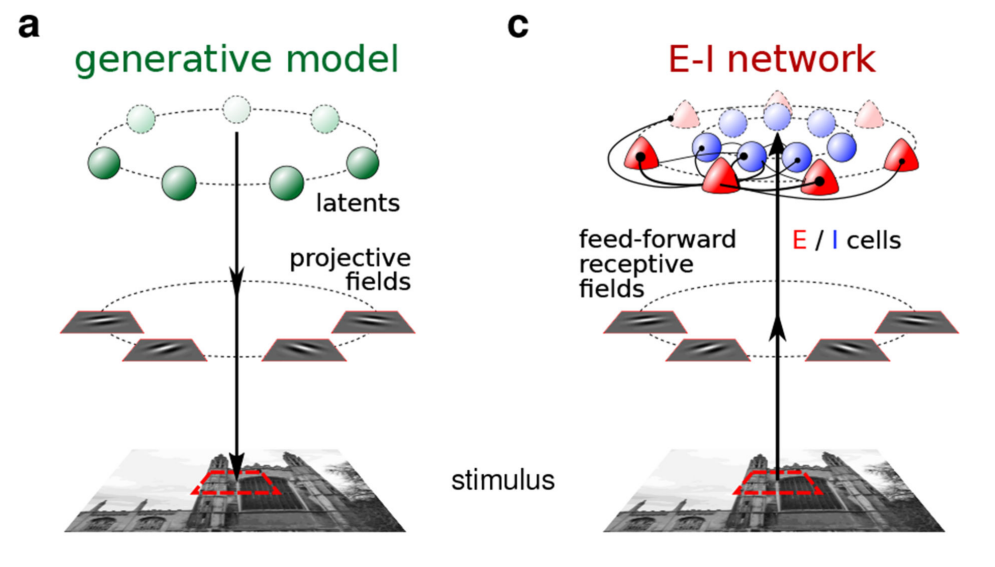
\includegraphics[width=0.90\textwidth]{04_antecedentes/figures/arquieche.png}
    \caption{
        % a, Esquema del GSM. Un parche de imagen se construye como una combinación lineal de un conjunto fijo de características localizadas y orientadas, similares a las de un filtro de Gabor.
        % b, proyección bidimensional de la distribución posterior sobre variables latentes dado un estímulo visual, calculada por el observador ideal bayesiano bajo el modelo generativo.
        El modelo generativo estadístico y el circuito neuronal correspondiente que implementa la inferencia probabilística basada en muestreo.
    }
    \label{fig:arquieche}
\end{figure}


\subsection{El modelo generativo (GSM)}
\label{subsec:echeveste_gsm}

Para especificar el problema computacional objetivo, los autores adoptan el \textbf{modelo de mezcla de escala gaussiana} (\acrfull{GSM}), un modelo generativo bien establecido que captura las estadísticas de parches de imágenes naturales \citep{echeveste2020cortical}. En este modelo, un parche de imagen $\mathbf{x} \in \mathbb{R}^{N_x}$ se genera como:

\begin{equation}
\mathbf{x} | \mathbf{y}, z \sim \mathcal{N}(z \mathbf{A} \mathbf{y}, \sigma_x^2 \mathbf{I})
\label{eq:gsm_likelihood}
\end{equation}

donde $\mathbf{y} \in \mathbb{R}^{N_y}$ son las variables latentes que representan intensidades de características visuales, $\mathbf{A} \in \mathbb{R}^{N_x \times N_y}$ es la matriz de \textit{campos proyectivos} (cuyas columnas son filtros tipo Gabor orientados, como se describió en la Sección~\ref{subsec:filtros_gabor}), $z \in \mathbb{R}$ es una variable de contraste global, y $\sigma_x^2$ es la varianza del ruido sensorial.

Las variables latentes siguen un prior gaussiano multivariado:

\begin{equation}
\mathbf{y} \sim \mathcal{N}(\mathbf{0}, \mathbf{C})
\label{eq:gsm_prior}
\end{equation}

donde $\mathbf{C}$ es la matriz de covarianza del prior, parametrizada como matriz circulante cuyos elementos varían suavemente en función de la diferencia angular entre las orientaciones preferidas de los campos proyectivos correspondientes.

Para modelar inferencia en una hipercolumna de V1, los campos proyectivos (columnas de $\mathbf{A}$) se eligen como filtros de Gabor orientados que difieren únicamente en su orientación, distribuidos uniformemente entre $-90^\circ$ y $90^\circ$, formando así una topología de anillo.

\begin{equation}
\mathbf{x} = z \cdot \mathbf{A}\mathbf{y} + \boldsymbol{\epsilon}
\label{eq:gsm}
\end{equation}

donde $\mathbf{y}$ son variables latentes (intensidades de características visuales como filtros de Gabor), $\mathbf{A}$ es la matriz de campos proyectivos, $z$ es una variable de contraste global, y $\boldsymbol{\epsilon}$ es ruido sensorial.

\subsubsection{Distribución posterior del observador ideal}

Bajo el \acrshort{GSM}, la distribución posterior sobre las variables latentes dado un parche de imagen y un contraste conocido tiene forma gaussiana:

\begin{equation}
P_{\text{GSM}}(\mathbf{y}|\mathbf{x}, z) = \mathcal{N}(\mathbf{y}; \boldsymbol{\mu}_{\text{GSM}}, \boldsymbol{\Sigma}_{\text{GSM}})
\label{eq:gsm_posterior}
\end{equation}

con media y covarianza posteriores dadas por:

\begin{equation}
\boldsymbol{\mu}_{\text{GSM}} = \frac{z}{\sigma_x^2} \boldsymbol{\Sigma}_{\text{GSM}} \mathbf{A}^\top \mathbf{x}
\label{eq:gsm_posterior_mean}
\end{equation}

\begin{equation}
\boldsymbol{\Sigma}_{\text{GSM}} = \left( \mathbf{C}^{-1} + \frac{z^2}{\sigma_x^2} \mathbf{A}^\top \mathbf{A} \right)^{-1}
\label{eq:gsm_posterior_cov}
\end{equation}

Nótese que la covarianza posterior \eqref{eq:gsm_posterior_cov} decrece con $z^2$: a mayor contraste, menor incertidumbre en la estimación. Por su parte, la media posterior \eqref{eq:gsm_posterior_mean} depende del contraste de manera que para contrastes altos converge hacia el valor verdadero de las variables latentes, mientras que para contrastes bajos se acerca a la media del prior (cero). Estas propiedades, mayor precisión y mejores estimaciones con mayor contraste, son características que la red neuronal deberá reproducir.

En el modelo, el contraste $z$ se aproxima con su valor verdadero $z^*$, dado que es un único escalar cuya inferencia integra información de todos los píxeles:

\begin{equation}
P_{\text{GSM}}(\mathbf{y}|\mathbf{x}) \approx P_{\text{GSM}}(\mathbf{y}|\mathbf{x}, z^*)
\label{eq:gsm_marginal}
\end{equation}


\subsubsection{Transformación de variables latentes a potenciales de membrana}

Siguiendo trabajos previos, los potenciales de membrana $u_i$ se toman como una transformación débilmente no lineal de las activaciones de características visuales $y_i$:

\begin{equation}
u_i(y_i) = \left[ \alpha_{\text{nl}} y_i + \beta_{\text{nl}} \right]_+^{\gamma_{\text{nl}}}
\label{eq:latent_to_membrane}
\end{equation}

donde $[\cdot]_+$ denota la función de rectificación (threshold-linear), y $\alpha_{\text{nl}}$, $\beta_{\text{nl}}$, $\gamma_{\text{nl}}$ son respectivamente la escala, línea base y exponente de la transformación. Esta transformación permite que los potenciales de membrana representen las intensidades de características mientras respetan restricciones biológicas como la no-negatividad.

\subsection{Dinámica neuronal}
\label{subsec:echeveste_dinamica}

El modelo implementa una \textbf{red supralineal estabilizada} \acrfull{SSN}, una arquitectura que captura propiedades esenciales de los circuitos corticales. La red consiste en $N_E$ neuronas excitatorias y $N_I$ neuronas inhibitorias. La dinámica de cada neurona $i$ está controlada por:

\begin{equation}
\tau_i \frac{du_i}{dt} = -u_i(t) + h_i(t) + \sum_j W_{ij} r_j(t) + \eta_i(t)
\label{eq:ssn_dynamics}
\end{equation}

donde $u_i$ es el potencial de membrana, $h_i$ es la entrada feedforward dependiente del estímulo, $W_{ij}$ son los pesos sinápticos recurrentes, $r_j$ es la tasa de disparo de la neurona $j$, y $\eta_i(t)$ es ruido de proceso correlacionado temporalmente.

\subsubsection{Función de transferencia supralineal}

Las tasas de disparo se derivan de los potenciales de membrana mediante una función de transferencia supralineal:

\begin{equation}
r_i(t) = k \left[ u_i(t) \right]_+^n
\label{eq:firing_rate}
\end{equation}

donde $[\cdot]_+$ denota rectificación ($[x]_+ = \max(0, x)$), $k$ es un factor de escala, y $n > 1$ es el exponente supralineal (ambos parámetros fijos). Esta no linealidad es consistente con observaciones experimentales en neuronas corticales y resulta fundamental para las propiedades de estabilización del circuito. El término ``supralineal'' indica que la función es convexa para potenciales positivos, lo que produce respuestas que crecen más rápido que linealmente con la entrada.

\subsubsection{Parametrización de la conectividad (topología de anillo)}

Dado que la red debe exhibir la misma simetría circular que el GSM estructurado en anillo, la conectividad recurrente se parametriza de forma rotacionalmente simétrica. Las neuronas se organizan en pares E-I alrededor de un ``anillo'' según sus orientaciones preferidas, y la conectividad es una función gaussiana circular de la diferencia de orientación entre células.

Específicamente, cada cuadrante de la matriz de pesos ($E \rightarrow E$, $E \rightarrow I$, $I \rightarrow E$, $I \rightarrow I$) se define como:

\begin{equation}
W_{XY}(\theta_i, \theta_j) = a_{XY} \exp\left( \frac{\cos(2(\theta_i - \theta_j)) - 1}{d_{XY}^2} \right)
\label{eq:weight_parametrization}
\end{equation}

donde $X, Y \in \{E, I\}$, $\theta_i = \pi i / N_{E/I}$ es la orientación preferida de la $i$-ésima neurona E/I, $a_{XY}$ controla la amplitud de las conexiones, y $d_{XY}$ controla su ancho espacial.

Para respetar el \textbf{principio de Dale}, se imponen las siguientes restricciones sobre las amplitudes:
\begin{itemize}
    \item $a_{XE} > 0$ para $X \in \{E, I\}$ (conexiones desde neuronas excitatorias son positivas)
    \item $a_{XI} < 0$ para $X \in \{E, I\}$ (conexiones desde neuronas inhibitorias son negativas)
\end{itemize}

Esta parametrización circulante reduce drásticamente el número de parámetros libres: en lugar de optimizar todos los elementos de la matriz de pesos, para esta sección solo se optimizan 8 parámetros ($a_{XY}$ y $d_{XY}$ para cada cuadrante).

\subsubsection{Ruido de proceso}

El ruido de proceso $\eta_i(t)$ modela la variabilidad intrínseca y extrínseca de la actividad neuronal (entradas de otras áreas cerebrales, fluctuaciones de canal, etc.). Crucialmente, este ruido es \textbf{independiente del estímulo}, lo que implica que la red debe usar sus dinámicas recurrentes para moldear la variabilidad de manera apropiada para cada entrada.

El ruido es gaussiano con media cero y correlaciones espaciales y temporales:

\begin{equation}
\langle \eta_i(t) \rangle = 0, \quad \langle \eta_i(t) \eta_j(t+s)^\top \rangle = \Sigma_{ij}^\eta \exp(-|s|/\tau_\eta)
\label{eq:noise_correlation}
\end{equation}

% donde $\tau_\eta$ es la escala temporal del ruido y $\boldsymbol{\Sigma}^\eta$ es la matriz de covarianza espacial instantánea, también parametrizada de forma circulante con 4 parámetros adicionales ($\sigma_E$, $\sigma_I$, $\rho$, $d_\sigma$).

donde $\tau_\eta$ es la escala temporal del ruido y $\boldsymbol{\Sigma}^\eta$ es la matriz de covarianza espacial instantánea.

La covarianza espacial del ruido también se parametriza de forma circulante:

\begin{equation}
\Sigma_{EE/II}^\eta(\theta_i, \theta_j) = \sigma_{E/I}^2 \exp\left( \frac{\cos(2(\theta_i - \theta_j)) - 1}{d_\sigma^2} \right)
\label{eq:noise_cov_same}
\end{equation}

\begin{equation}
\Sigma_{EI}^\eta(\theta_i, \theta_j) = \rho \sigma_E \sigma_I \exp\left( \frac{\cos(2(\theta_i - \theta_j)) - 1}{d_\sigma^2} \right)
\label{eq:noise_cov_cross}
\end{equation}

donde $\sigma_E, \sigma_I > 0$ son las desviaciones estándar del ruido para poblaciones E e I, $\rho$ es el coeficiente de correlación entre ruido E e I, y $d_\sigma$ controla el ancho espacial de las correlaciones de ruido. Esto introduce 4 parámetros adicionales para el entrenamiento.

\subsubsection{Entrada feedforward}

La entrada dependiente del estímulo a cada neurona se obtiene aplicando un filtro lineal al estímulo seguido de una no linealidad estática:

\begin{equation}
h_i(t) = \left[ \alpha_h \left( \beta_h + \sum_j W_{ij}^{ff} x_j(t) \right) \right]_+^{\gamma_h}
\label{eq:feedforward_input}
\end{equation}

donde $\mathbf{x}(t)$ es el estímulo (parche de imagen), $\mathbf{W}^{ff}$ es la matriz de campos receptivos feedforward, y $\alpha_h$, $\beta_h$, $\gamma_h$ son respectivamente la escala, línea base y exponente de la no linealidad de entrada, así agregando estos últimos 3 parámetros.

Los campos receptivos feedforward se fijan idénticos a los campos proyectivos del \acrshort{GSM}:

\begin{equation}
\mathbf{W}^{ff} = \frac{1}{15} [\mathbf{A} \; \mathbf{A}]^\top
\label{eq:feedforward_weights}
\end{equation}

donde $[\mathbf{A} \; \mathbf{A}]$ denota la concatenación de $\mathbf{A}$ consigo misma (para proporcionar la misma entrada a cada par E-I).

\subsubsection{Correspondencia entre red y modelo generativo}

Existe una correspondencia uno-a-uno entre las variables latentes del \acrshort{GSM} y las neuronas excitatorias de la red: el potencial de membrana de cada célula E representa la intensidad de una característica visual diferente. Las neuronas inhibitorias se tratan como unidades auxiliares no explícitamente restringidas por el objetivo computacional, pero esenciales para la estabilidad y las dinámicas del circuito.

En resumen, la red tiene \textbf{15 parámetros libres}:
\begin{itemize}
    \item 8 para la matriz de pesos ($a_{XY}$, $d_{XY}$ para cada cuadrante)
    \item 4 para la covarianza del ruido ($\sigma_E$, $\sigma_I$, $\rho$, $d_\sigma$)
    \item 3 para la no linealidad de entrada ($\alpha_h$, $\beta_h$, $\gamma_h$)
\end{itemize}

\subsection{Entrenamiento para muestreo}
\label{subsec:echeveste_entrenamiento}

El aspecto técnicamente más novedoso del trabajo de \citeauthor{echeveste2020cortical} es el procedimiento de optimización. A diferencia de enfoques tradicionales que entrenan redes para producir respuestas promedio correctas, aquí el objetivo es que la \textit{distribución} de respuestas de la red coincida con la distribución posterior del modelo generativo.

\subsubsection{Momentos objetivo}

Para cada estímulo de entrenamiento $\mathbf{x}^{(\alpha)}$, se computan los momentos objetivo de la posterior bajo el \acrshort{GSM}. Estos ``momentos objetivo'' se definen transformando los momentos de la posterior sobre $\mathbf{y}$ al espacio de potenciales de membrana $\mathbf{u}$ mediante la ecuación \ref{eq:latent_to_membrane}:

\begin{equation}
\boldsymbol{\mu}_{\text{tgt}}^{(\alpha)} = \int \mathbf{u}(\mathbf{y}) \, P_{\text{GSM}}(\mathbf{y}|\mathbf{x}^{(\alpha)}) \, d\mathbf{y}
\label{eq:target_mean}
\end{equation}

\begin{equation}
\boldsymbol{\Sigma}_{\text{tgt}}^{(\alpha)} = \int \mathbf{u}(\mathbf{y}) \mathbf{u}^\top(\mathbf{y}) \, P_{\text{GSM}}(\mathbf{y}|\mathbf{x}^{(\alpha)}) \, d\mathbf{y} - \boldsymbol{\mu}_{\text{tgt}}^{(\alpha)} (\boldsymbol{\mu}_{\text{tgt}}^{(\alpha)})^\top
\label{eq:target_cov}
\end{equation}

Estas ecuaciones calculan la media \eqref{eq:target_mean} y la covarianza \eqref{eq:target_cov} objetivo que la red debe reproducir. En ambos casos, las integrales representan valores esperados bajo la distribución posterior $P_{\text{GSM}}(\mathbf{y}|\mathbf{x}^{(\alpha)})$.
La media objetivo $\boldsymbol{\mu}_{\text{tgt}}^{(\alpha)}$ es el promedio de los potenciales de membrana ponderado por la probabilidad de cada configuración de variables latentes, mientras que la covarianza objetivo $\boldsymbol{\Sigma}_{\text{tgt}}^{(\alpha)}$ cuantifica la dispersión esperada alrededor de dicha media. Intuitivamente, estos momentos definen la distribución que la actividad fluctuante de la red debe aproximar mediante muestreo temporal.

\subsubsection{Conjunto de entrenamiento}

El conjunto de entrenamiento consiste en solo cinco parches de imagen con el mismo contenido pero diferentes niveles de contraste:

\begin{equation}
\mathbf{x}^{(\alpha)} = z^{(\alpha)} \mathbf{A} \bar{\mathbf{y}}
\label{eq:training_stimuli}
\end{equation}

con $\alpha = 1, \ldots, 5$ y $z^{(\alpha)} \in \{0, 0.125, 0.25, 0.5, 1.0\}$. El contenido $\bar{\mathbf{y}}$ es una función gaussiana de $27°$ de ancho centrada en $0°$ (una única orientación dominante). Gracias a la parametrización rotacionalmente invariante, entrenar en un estímulo equivale a entrenar en todas sus posibles rotaciones.

\begin{figure}[!ht]
    \centering
    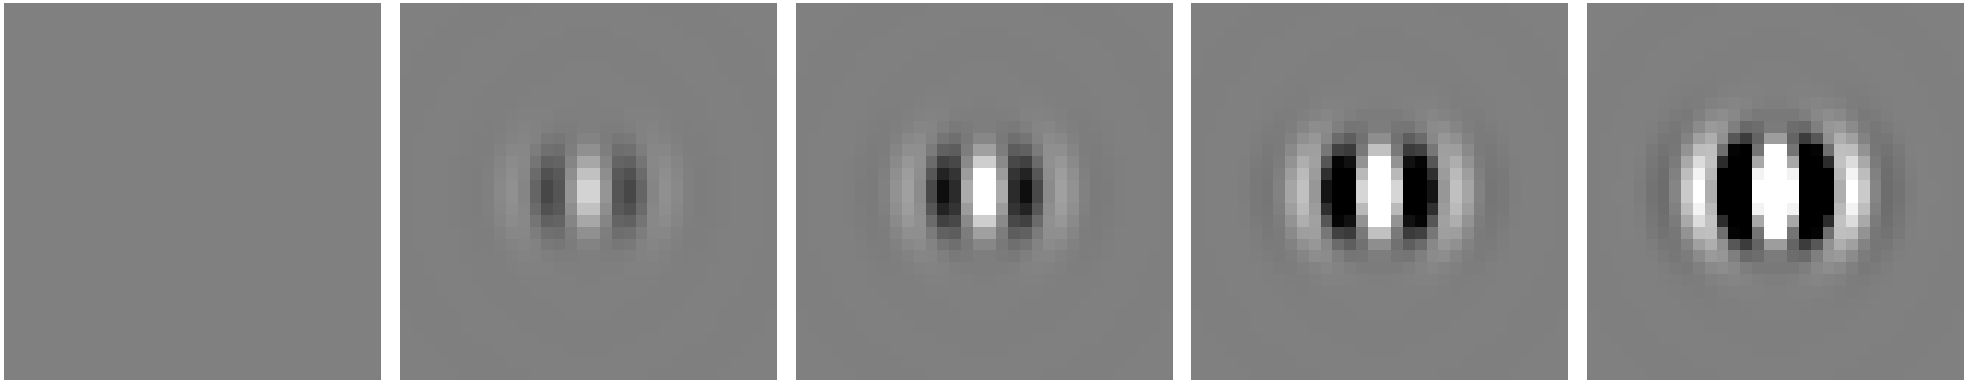
\includegraphics[width=0.85\textwidth]{05_modelos/figures/training_stimuli_contrast.png}
    \caption{
        Conjunto de entrenamiento del modelo de Echeveste. Los cinco estímulos comparten el mismo contenido $\bar{\mathbf{y}}$ (gaussiana de 27° centrada en 0°) 
        pero difieren en su nivel de contraste $z^{(\alpha)} \in \{0, 0.125, 0.25, 0.5, 1.0\}$.
    }
    \label{fig:training_stimuli}
\end{figure}

\subsubsection{Función de costo}

El entrenamiento de la red consiste en ajustar parámetros de modo que la distribución de actividad neuronal reproduzca las estadísticas deseadas. Formalmente, esto se logra minimizando una función de costo $\mathcal{F}$ que cuantifica la discrepancia entre el comportamiento actual de la red y el objetivo:

\begin{equation}
\mathcal{F} = \sum_\alpha \left( \epsilon_{\text{mean}} \phi_{\text{mean}}^{(\alpha)} + \epsilon_{\text{var}} \phi_{\text{var}}^{(\alpha)} + \epsilon_{\text{cov}} \phi_{\text{cov}}^{(\alpha)} + \epsilon_{\text{slow}} \phi_{\text{slow}}^{(\alpha)} \right)
\label{eq:cost_function}
\end{equation}

donde los coeficientes $\epsilon$ controlan la importancia relativa de cada término. 

Los primeros tres términos penalizan diferencias entre los momentos de la distribución de respuestas de la red (promediados sobre una ventana temporal) y los momentos objetivo correspondientes:

\begin{equation}
\phi_{\text{mean}}^{(\alpha)} = \int_{T_{\min}}^{T_{\max}} \left\| \boldsymbol{\mu}^{(\alpha)}(t) - \boldsymbol{\mu}_{\text{tgt}}^{(\alpha)} \right\|_F^2 \, dt
\label{eq:cost_mean}
\end{equation}

\begin{equation}
\phi_{\text{var}}^{(\alpha)} = \int_{T_{\min}}^{T_{\max}} \left\| \boldsymbol{\sigma}^{(\alpha)}(t) - \boldsymbol{\sigma}_{\text{tgt}}^{(\alpha)} \right\|_F^2 \, dt
\label{eq:cost_var}
\end{equation}

\begin{equation}
\phi_{\text{cov}}^{(\alpha)} = \int_{T_{\min}}^{T_{\max}} \left\| \boldsymbol{\Sigma}^{(\alpha)}(t, 0) - \boldsymbol{\Sigma}_{\text{tgt}}^{(\alpha)} \right\|_F^2 \, dt
\label{eq:cost_cov}
\end{equation}

donde $\boldsymbol{\mu}^{(\alpha)}(t) = \langle \mathbf{u}(t) \rangle$ es la media across-trial de los potenciales de membrana, $\boldsymbol{\sigma}^{(\alpha)}(t) = \text{diag}(\boldsymbol{\Sigma}^{(\alpha)}(t, 0))$ es el vector de varianzas, $\boldsymbol{\Sigma}^{(\alpha)}(t, 0)$ es la matriz de covarianza instantánea, y $\|\cdot\|_F$ denota la norma de Frobenius.

El cuarto término es un costo de ``lentitud'' que penaliza la autocorrelación temporal de las respuestas, incentivando que muestras consecutivas sean estadísticamente independientes:

\begin{equation}
\phi_{\text{slow}}^{(\alpha)} = \int_0^{\tau_{\max}} \left\| \text{diag}(\mathbf{C}^{(\alpha)}(\tau)) \right\|_F^2 \, d\tau
\label{eq:cost_slow}
\end{equation}

donde $\mathbf{C}^{(\alpha)}(\tau) = \text{corr}(\mathbf{u}(t), \mathbf{u}(t + \tau))$ es la matriz de autocorrelación temporal.

\subsubsection{Procedimiento de optimización}

\textbf{Fase 1 (estocástica):} Se emplea un método de gradiente estocástico, una técnica de optimización donde el gradiente de la función de costo se estima a partir de un subconjunto de datos en lugar de calcularse exactamente. En este caso, se utilizan $N_{\text{trial}} = 50$ trials por estímulo para estimar los momentos de las respuestas, introduciendo variabilidad en las estimaciones del gradiente pero permitiendo un cálculo computacionalmente más eficiente. Se realizan 250 iteraciones del optimizador \acrshort{ADAM}. Durante esta fase, el inicio de la ventana de promediado $T_{\min}$ se ``recuece'' (\textit{annealing}) sistemáticamente desde $T_{\min} = 0$ ms hasta $T_{\max} - 50$ ms, incentivando dinámicas de muestreo rápidas desde el inicio del estímulo.


\textbf{Fase 2 (determinística):} Se continúa la optimización usando el optimizador \acrshort{L-BFGS-B} con el método de \acrfull{ADF} para calcular determinísticamente los momentos de la distribución de respuestas. Este método asume que la distribución conjunta espacio-temporal de potenciales de membrana es gaussiana, permitiendo obtener los momentos en forma cerrada.

La función de costo es no convexa, por lo que \citeauthor{echeveste2020cortical} verificaron la robustez de los resultados realizando 10 optimizaciones adicionales desde condiciones iniciales aleatorias, encontrando que todas las soluciones con costos comparables exhibían cualitativamente las mismas propiedades dinámicas.

\subsection{Propiedades emergentes}
\label{subsec:echeveste_propiedades}

Notablemente, la red optimizada exhibe un conjunto de propiedades dinámicas que emergen como consecuencia del objetivo de muestreo, sin ser explícitamente impuestas durante el entrenamiento:

\textbf{Variabilidad modulada por el estímulo:} La varianza de las respuestas neuronales decrece con el contraste del estímulo, reproduciendo observaciones experimentales en corteza visual. Este comportamiento refleja directamente las propiedades de la posterior del \acrshort{GSM}, donde mayor contraste implica menor incertidumbre.

\textbf{Transitorios inhibitorios:} Al inicio de un estímulo, la inhibición domina transitoriamente sobre la excitación, generando sobrepicos (\textit{overshoots}) en las tasas de disparo poblacionales seguidos de adaptación hacia un estado estacionario. La magnitud de estos transitorios escala con el contraste del estímulo.

\textbf{Oscilaciones gamma:} La actividad de la red exhibe oscilaciones en el rango gamma (30-80 Hz), detectables tanto en autocorrelogramas de neuronas individuales como en el potencial de campo local (LFP) simulado. Crucialmente, la frecuencia pico de las oscilaciones gamma aumenta con el contraste del estímulo, replicando hallazgos experimentales robustos en V1 de primates.

\subsection{Roles funcionales de las dinámicas}
\label{subsec:echeveste_roles}

\citeauthor{echeveste2020cortical} demostraron que estas propiedades dinámicas no son meros epifenómenos sino que cumplen roles funcionales específicos en la inferencia probabilística:

\subsubsection{Rol de las oscilaciones: mejora del tiempo de mezcla}

Las oscilaciones gamma implementan una forma de muestreo fuera del equilibrio que acelera la exploración del espacio de estados. En algoritmos de muestreo clásicos como Langevin, la dinámica es reversible temporalmente, lo que limita la velocidad con la que muestras consecutivas se vuelven estadísticamente independientes (``tiempo de mezcla''). Las trayectorias oscilatorias de la red optimizada permiten que muestras consecutivas cubran una región más amplia del espacio, reduciendo la correlación temporal y efectivamente aumentando el número de muestras independientes por unidad de tiempo.

Finalmente, la red optimizada alcanza convergencia a la distribución objetivo un orden de magnitud más rápido que un muestreador de Langevin equivalente, un método estándar de muestreo estocástico donde las muestras se generan mediante difusión gradual hacia la distribución objetivo, pero cuya dinámica reversible limita la velocidad de exploración del espacio de estados.

\subsubsection{Rol de los transitorios: reducción del tiempo de burn-in}

Los transitorios aceleran la convergencia de las muestras hacia la distribución estacionaria correcta al inicio de la estimulación (reducción del ``burn-in''). En lugar de difundir lentamente desde un estado inicial arbitrario, las respuestas transitorias rápidamente ``saltan'' hacia la región de alta probabilidad del espacio posterior.

El análisis teórico muestra que, para un estimador que promedia muestras en una ventana temporal finita, la trayectoria óptima que minimiza el error de estimación debe exhibir sobrepicos (overshoots) cuya magnitud escala con el valor objetivo. Los transitorios observados en la red optimizada reproducen cualitativamente esta predicción teórica.

Notablemente, \citeauthor{echeveste2020cortical} validaron esta predicción analizando datos experimentales publicados de V1 en mono despierto, encontrando una correlación positiva entre la magnitud del sobrepico transitorio y el cambio en la tasa de disparo estacionaria, consistente con las predicciones del modelo.


\subsection{Limitaciones y extensiones}
\label{subsec:echeveste_limitaciones}

La principal limitación del modelo de Echeveste para los propósitos de este trabajo es su restricción a \textbf{procesamiento unimodal}. El modelo fue diseñado para representar inferencia sobre características visuales de un único parche de imagen, sin considerar la integración de información de múltiples modalidades sensoriales ni el problema de la inferencia causal.


Otras limitaciones incluyen la arquitectura simplificada de hipercolumna (topología de anillo) que limita la generalización a estímulos más complejos y la ausencia de mecanismos de plasticidad sináptica (en simulación) o aprendizaje continuo. Es importante notar que, si bien la red exhibe una rica dinámica temporal gracias a sus conexiones recurrentes (donde la actividad presente depende de estados anteriores), esto no implica plasticidad en el sentido biológico de reconfiguración sináptica. En el modelo, los pesos sinápticos se determinan mediante un algoritmo de optimización externo (como ADAM o L-BFGS-B) antes de la ejecución ; una vez que la red comienza a realizar inferencia, estos pesos permanecen fijos y no se adaptan a nuevos estímulos o cambios en el entorno. Finalmente, la aproximación del contraste con su valor verdadero evita abordar el problema de la inferencia jerárquica completa.


Sin embargo, el marco teórico y las técnicas de optimización desarrolladas son, en principio, generalizables a arquitecturas más complejas. La metodología de entrenar redes con restricciones biológicas para que sus distribuciones de respuesta coincidan con posteriors objetivo podría extenderse a modelos generativos multimodales que incluyan estructura causal. Esta extensión constituye la dirección que motivó inicialmente el presente trabajo.

% =============================================================================
% SECCIÓN 3: OBJETIVO DEL PRESENTE TRABAJO
% =============================================================================

% \section{Objetivo del presente trabajo}
% \label{sec:objetivo}

% La revisión presentada en las secciones anteriores revela una brecha significativa en el modelado computacional de la integración multisensorial. Por un lado, modelos como el de \citet{cuppini2017biologically} capturan la arquitectura funcional de la integración audiovisual y la inferencia causal, pero emplean dinámicas de tasa deterministas que no reflejan las propiedades estocásticas y oscilatorias de la actividad cortical real. Por otro lado, el modelo de \citet{echeveste2020cortical} demuestra que redes neuronales con restricciones biológicas pueden implementar inferencia probabilística mediante muestreo, exhibiendo dinámicas corticales realistas, pero está limitado al procesamiento de una única modalidad sensorial. Además de estas diferencias conceptuales, existe una barrera práctica donde cada modelo ha sido implementado de manera independiente, en distintos lenguajes de programación y con estructuras de código incompatibles, dificultando su comparación sistemática y cualquier intento de integración.

% En nuestros inicios, nuestra principal pregunta fue si era posible combinar lo mejor de ambos trabajos: construir un modelo de integración multisensorial que resuelva el problema de inferencia causal audiovisual mientras exhibe las dinámicas corticales biológicamente plausibles que caracterizan al modelo de Echeveste. Un modelo así tendría implicaciones profundas tanto teóricas, demostrando que los principios de muestreo neuronal pueden extenderse al dominio multisensorial, como prácticas, permitiendo conectar predicciones del modelo con observaciones electrofisiológicas reales.

% Sin embargo, realizar esta idea no es una tarea que pueda abordarse en un único trabajo. La fusión de estos modelos requiere resolver múltiples desafíos técnicos y conceptuales que deben abordarse de manera sistemática. El presente trabajo representa el primer paso en esta dirección, al sentar las bases computacionales necesarias para que dicha fusión sea posible en investigaciones futuras.

% \subsection{La visión y el camino hacia ella}
% \label{subsec:vision}

% La visión a largo plazo que motiva este trabajo es el desarrollo de modelos de integración multisensorial que combinen la arquitectura multimodal del modelo de Cuppini con las dinámicas corticales realistas del modelo de Echeveste. Un modelo así permitiría estudiar cómo fenómenos como el efecto ventrílocuo emergen de circuitos neuronales que no solo integran información de múltiples modalidades, sino que lo hacen mediante mecanismos de muestreo estocástico biológicamente plausibles.

% Para alcanzar esta visión, es necesario primero disponer de una implementación del modelo de Echeveste dentro de un framework que facilite su extensión y comparación con otros modelos. El framework Scikit-NeuroMSI, descrito en el Capítulo~\ref{chapter:scikit_neuromsi}, representa la plataforma ideal para este propósito: ya incluye implementaciones del modelo de Cuppini y de modelos bayesianos de inferencia causal, proporcionando la infraestructura necesaria para comparaciones sistemáticas.

% \subsection{Desafíos y extensiones necesarias}
% \label{subsec:desafios}

% El modelo de Echeveste introduce al framework un tipo de modelo cualitativamente diferente a los existentes en varios aspectos fundamentales.

% En primer lugar, existe una diferencia en el \textbf{dominio de representación}. Los modelos actualmente implementados en Scikit-NeuroMSI modelan la localización espacial de estímulos, con neuronas organizadas topográficamente según posiciones en el espacio externo (vía dorsal). En contraste, el modelo de Echeveste representa características visuales como la orientación de bordes, con neuronas organizadas según sus orientaciones preferidas en una hipercolumna de V1 (vía ventral). Esta diferencia implica que la integración de ambos enfoques requerirá considerar cómo diferentes tipos de representaciones corticales pueden interactuar en el contexto de la inferencia multisensorial.

% En segundo lugar, el modelo de Echeveste es inherentemente \textbf{estocástico} de una manera que resulta central para su función: sus propiedades más relevantes emergen precisamente de la distribución de actividad neuronal y su evolución temporal. Los transitorios, las oscilaciones gamma, y la variabilidad trial-a-trial no son fenómenos secundarios sino características centrales que el modelo utiliza activamente para implementar inferencia probabilística mediante muestreo.

% Esta diferencia tiene implicaciones directas para la implementación. Será necesario desarrollar herramientas para visualizar y analizar la evolución temporal de los estados neuronales, calcular autocorrelaciones temporales, analizar espectros de potencia para identificar oscilaciones, y comparar la distribución de respuestas con los momentos objetivo derivados del modelo generativo.

% Otra extensión necesaria es la implementación del \textbf{modelo generativo GSM} que define el problema de inferencia que la red debe resolver. Este modelo generativo no existe actualmente en el framework y su implementación es condición necesaria para poder entrenar la red y validar que sus respuestas aproximan correctamente la inferencia bayesiana óptima.

% \subsection{Contribución del presente trabajo}
% \label{subsec:contribucion}

% El presente trabajo aborda estos desafíos mediante la implementación completa del modelo de Echeveste dentro del framework Scikit-NeuroMSI. Esta implementación incluye la arquitectura de red con sus poblaciones excitatorias e inhibitorias, la parametrización de conectividad en anillo, el modelo generativo GSM con el cálculo de momentos objetivo, y el procedimiento de entrenamiento para muestreo.

% Junto con el modelo, el trabajo desarrolla bases para las herramientas de análisis necesarias para estudiar modelos con dinámicas temporales relevantes. Estas herramientas permitirán visualizar la evolución de los potenciales de membrana, calcular espectros de potencia para identificar oscilaciones, y comparar estadísticas de las respuestas con los valores objetivo.

% La validación de la implementación verificará que el modelo reproduce las propiedades reportadas en el trabajo original: convergencia de los momentos de respuesta hacia los momentos objetivo, variabilidad modulada por contraste, y presencia de las dinámicas temporales características.

% Es importante delimitar claramente lo que este trabajo \textbf{no aborda}. La fusión del modelo de Echeveste con el modelo de Cuppini, la implementación de inferencia causal multisensorial, y la validación contra datos experimentales de integración audiovisual quedan como direcciones de investigación futura. El presente trabajo se enfoca exclusivamente en sentar las bases técnicas que harán posibles estas extensiones, reconociendo que una implementación correcta y validada del modelo unimodal de Echeveste es condición necesaria para cualquier desarrollo posterior hacia el procesamiento multisensorial con dinámicas corticales realistas.